\documentclass[border=1pt]{standalone}
\usepackage{pgfplots}
\usepgfplotslibrary{groupplots,fillbetween}
\usepackage{animate}

\usepackage{pgf}
\usepackage{tikz}

\usetikzlibrary{fit}
\usetikzlibrary{positioning}
\usetikzlibrary{arrows}
\usetikzlibrary{automata}
\usetikzlibrary{backgrounds}
\usetikzlibrary{shapes.misc}

% https://tex.stackexchange.com/questions/118223/drawing-little-semicircle-to-show-that-two-intersecting-lines-are-not-connected
\usetikzlibrary{calc}

% \intersect{<p1>}{<p2>}{<q1>}{<q2>}
% draws the line p1--p2, showing a little semicircle
% where it intersects the line q1--q2.
\newcommand\intersect[4]{
  \draw let \p{c} = (intersection of #1--#2 and #3--#4) in
    (#1) -- ($(\p{c})!0.75mm!(#1)$) 
    to[bend right=90] ($(\p{c})!0.75mm!(#2)$) -- (#2)
}


\begin{document}    
  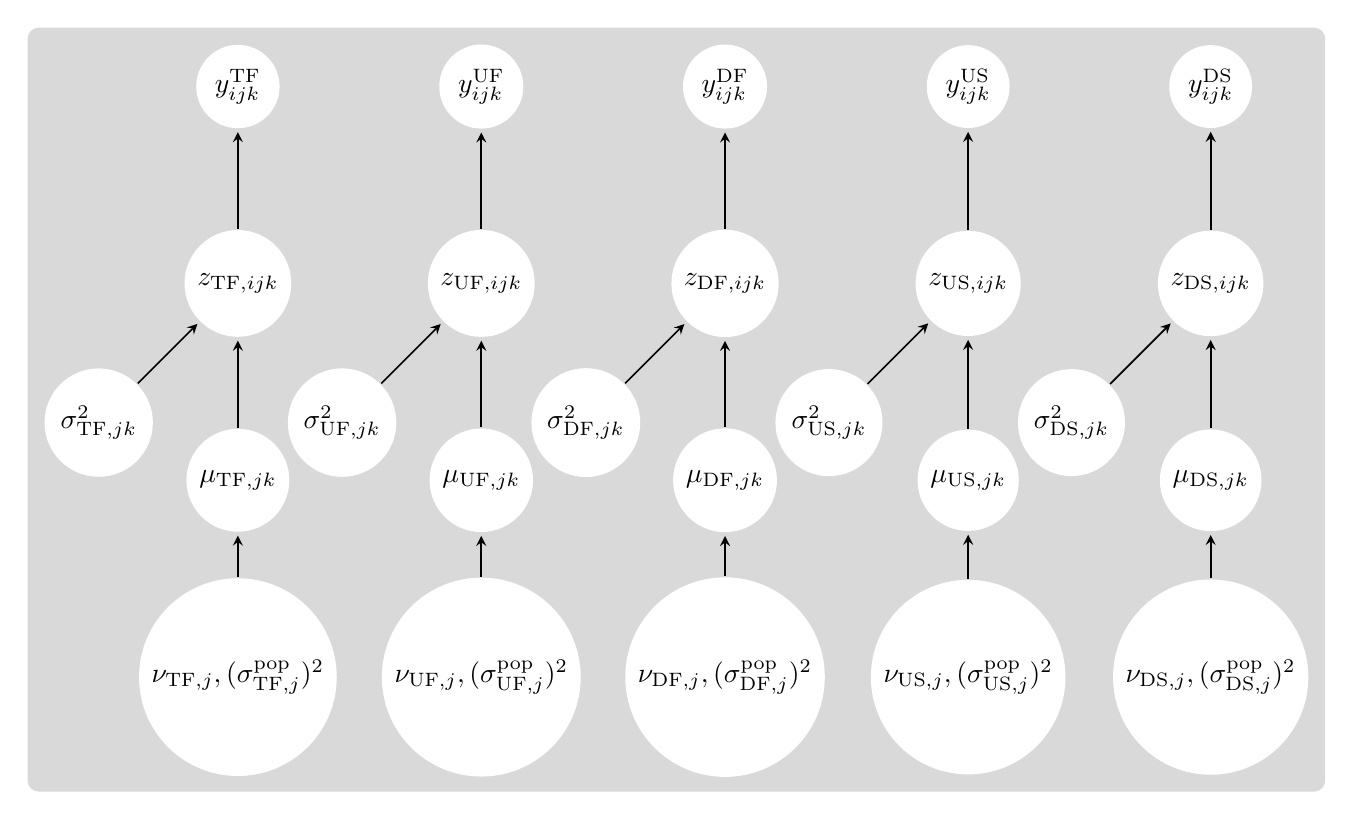
\begin{tikzpicture}[
            > = stealth, % arrow head style
            shorten > = 1pt, % don't touch arrow head to node
            auto,
            node distance = 2.5cm, % distance between nodes
            semithick % line style
            ]

        \tikzstyle{every state}=[
            draw = none,
            thick,
            fill = white,
            minimum size = 4mm
        ]F


	% data level
	\node[state] (Y) [] {$y^{\mathrm{UF}}_{ijk}$};
	\node[state] (Y2) [left =2cm of Y] {$y^{\mathrm{TF}}_{ijk}$};
       	\node[state] (Y3) [right  =2cm of Y] {$y^{\mathrm{DF}}_{ijk}$};
         \node[state] (Y4) [right  =2cm of Y3] {$y^{\mathrm{US}}_{ijk}$};
         \node[state] (Y5) [right  =2cm of Y4] {$y^{\mathrm{DS}}_{ijk}$};
    

        
        % parameters
         \node[state] (A) [below of = Y] {$z_{\mathrm{UF},ijk}$};          
         \path[->] (A) edge node {} (Y);
         
          \node[state] (MU) [below of = A] {$\mu_{\mathrm{UF},jk}$};
         \node[state] (SIG) [below left of = A] {$\sigma_{\mathrm{UF},jk}^2$};
         
         \path[->] (SIG) edge node {} (A);       
         \path[->] (MU) edge node {} (A);       
         
         \node[state] (H) [below of = MU] {$\nu_{\mathrm{UF},j},(\sigma^\mathrm{pop}_{\mathrm{UF},j})^2$};
         \path[->] (H) edge node {} (MU);       
         
         
         % parameters
         \node[state] (A2) [below of = Y2] {$z_{\mathrm{TF},ijk}$};          
         \path[->] (A2) edge node {} (Y2);
         
          \node[state] (MU2) [below of = A2] {$\mu_{\mathrm{TF},jk}$};
         \node[state] (SIG2) [below left of = A2] {$\sigma_{\mathrm{TF},jk}^2$};
         
         \path[->] (SIG2) edge node {} (A2);       
         \path[->] (MU2) edge node {} (A2);       
         
         \node[state] (H2) [below of = MU2] {$\nu_{\mathrm{TF},j},(\sigma^\mathrm{pop}_{\mathrm{TF},j})^2$};
         \path[->] (H2) edge node {} (MU2);       

         % parameters
         \node[state] (A3) [below of = Y3] {$z_{\mathrm{DF},ijk}$};          
         \path[->] (A3) edge node {} (Y3);
         
          \node[state] (MU3) [below of = A3] {$\mu_{\mathrm{DF},jk}$};
         \node[state] (SIG3) [below left of = A3] {$\sigma_{\mathrm{DF},jk}^2$};
         
         \path[->] (SIG3) edge node {} (A3);       
         \path[->] (MU3) edge node {} (A3);       
         
         \node[state] (H3) [below of = MU3] {$\nu_{\mathrm{DF},j},(\sigma^\mathrm{pop}_{\mathrm{DF},j})^2$};
         \path[->] (H3) edge node {} (MU3);      

                   % parameters
         \node[state] (A4) [below of = Y4] {$z_{\mathrm{US},ijk}$};          
         \path[->] (A4) edge node {} (Y4);
         
          \node[state] (MU4) [below of = A4] {$\mu_{\mathrm{US},jk}$};
         \node[state] (SIG4) [below left of = A4] {$\sigma_{\mathrm{US},jk}^2$};
         
         \path[->] (SIG4) edge node {} (A4);       
         \path[->] (MU4) edge node {} (A4);       
         
         \node[state] (H4) [below of = MU4] {$\nu_{\mathrm{US},j},(\sigma^\mathrm{pop}_{\mathrm{US},j})^2$};
         \path[->] (H4) edge node {} (MU4);      
         
                  % parameters
         \node[state] (A5) [below of = Y5] {$z_{\mathrm{DS},ijk}$};          
         \path[->] (A5) edge node {} (Y5);
         
          \node[state] (MU5) [below of = A5] {$\mu_{\mathrm{DS},jk}$};
         \node[state] (SIG5) [below left of = A5] {$\sigma_{\mathrm{DS},jk}^2$};
         
         \path[->] (SIG5) edge node {} (A5);       
         \path[->] (MU5) edge node {} (A5);       
         
         \node[state] (H5) [below of = MU5] {$\nu_{\mathrm{DS},j},(\sigma^\mathrm{pop}_{\mathrm{DS},j})^2$};
         \path[->] (H5) edge node {} (MU5);      
                                           
          \begin{scope}[on background layer]
   \node [fit=(SIG2) (Y) (H5), fill= gray!30, rounded corners, inner sep=.2cm] {};
 \end{scope}
                                 
  \end{tikzpicture}

  
  \end{document}